\section[VCS]{Visual Cryptographic Scheme}
En esta sección detallaremos el funcionamiento de los dos algoritmos de VCS:
\textbf{DVCS}(\textsl{Deterministic Visual Cryptographic Scheme}) y
\textbf{PVCS}(\textsl{Probabilistic Visual Cryptographic Scheme}).

Así como las condiciones que han de cumplir las \textsl{matrices base} sobre las
cuales estriban estos algoritmos.

Como ya comentamos, ambos algoritmos se estiban en un par matrices denominadas
``matrices base'' para transformar cada píxel de la imagen original en un
\textbf{superpíxel} de la sombra. Denominamos \textsl{superpíxel} al los píxeles
que representarán al píxel original en las sombras y la imagen recuperada. Éste
está compuesto por varios píxeles normales, negros y blancos (de ahí su nombre).

Dependiendo del número de píxeles negros y blancos que tenga un superpíxel de la
imagen resultado, se verá más negruzco o más blancuzco. Los superpíxeles
negruzcos representarán a los píxeles negros de la imagen original, y viceversa.
Un ejemplo de esto puede verse en la figura \ref{fig:ejemploVCS}.

\begin{figure}[h]
	\centering
	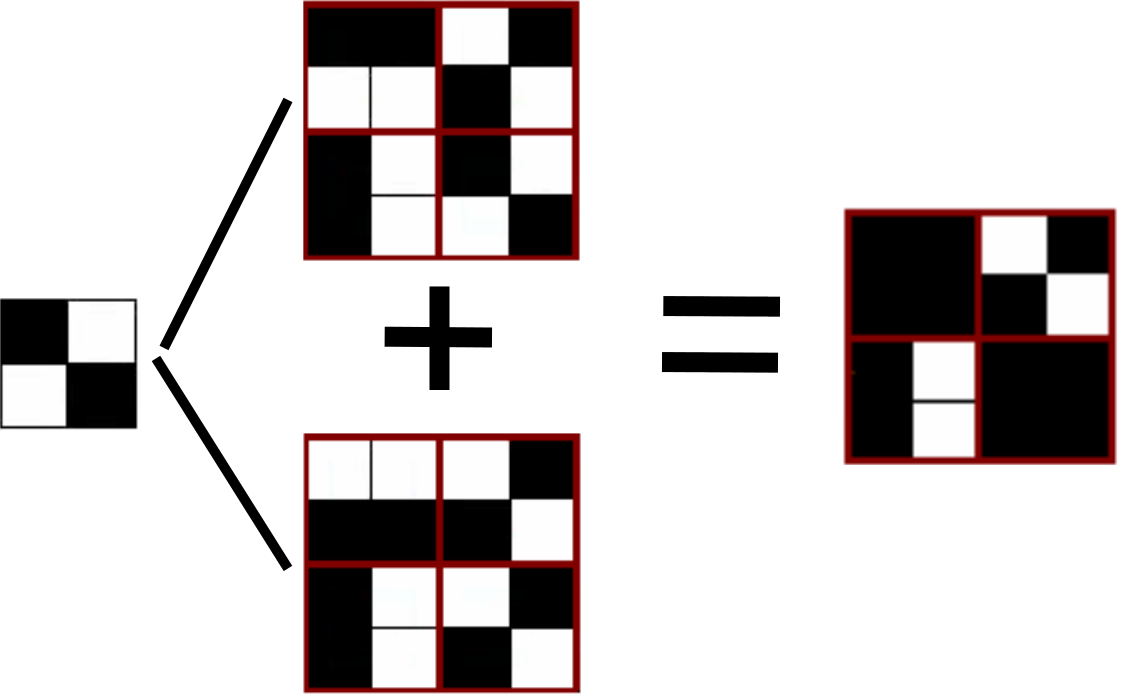
\includegraphics[width=0.7\textwidth]{images/ejemploVCS}
	\caption{Ejemplo que ilustra como la superposición de dos sombras da
		como resultado una imagen que imita los píxeles negros y blancos
		de la original}
	\label{fig:ejemploVCS}
\end{figure}

\subsection[DVCS]{Deterministic Visual Cryptographic Scheme}
El algoritmo DVCS recibe al adjetivo ``Determinista'' porque, en contraposición
a PVCS, los superpíxeles de la imagen resultante siempre tiene el mismo número
de píxeles negros y blancos, dependiendo de que sea un superpíxel negro o
blanco.

También se caracteriza por deformar las dimensiones de la imagen resultante, ya
que cada píxel de la imagen original se sustituye por $m$ píxeles en las
sombras. Estos $m$ píxeles se pueden distribuir en el superpíxel en una forma
cuadrática, siempre y cuando $m$ sea potencia de dos, así se conseguiría no
distorsionar el aspecto de la imagen original.

\subsubsection{Pseudocódigo}
\begin{algorithm}[H]
	\KwIn{\\Una imagen I secreta de $W\times H$\\Las matrices base $B_0$ y $B_1$}
	\KwResult{\\N sombras $S_i$ de tamaño $m\times W\times H$}

	\For{all pixel $px$ in I}{
		\eIf{$px$ == blanco}{
			1. Seleccionar una permutación $B^p_0$ aleatoria de $B_0$\;

			2. Añadir la columna i-ésima de $B^p_0$ ($m$ píxeles) al
			super-píxel de la i-ésima sombra $S_i$\;
		}{
			1. Seleccionar una permutación $B^p_1$ aleatoria de $B_1$\;

			2. Añadir la columna i-ésima de $B^p_0$ ($m$ píxeles) al
			super-píxel de la i-ésima sombra $S_i$\;
		}
	}
	\Return{$[S_1,S_2,\cdots,S_N]$}
	\caption{DVCS}
	\label{alg:DVCS}
\end{algorithm}
\newpage
\subsubsection{Ejemplos}
\begin{figure}[ht]
	\centering
	\begin{subfigure}[t]{0.9\textwidth}
		\centering
		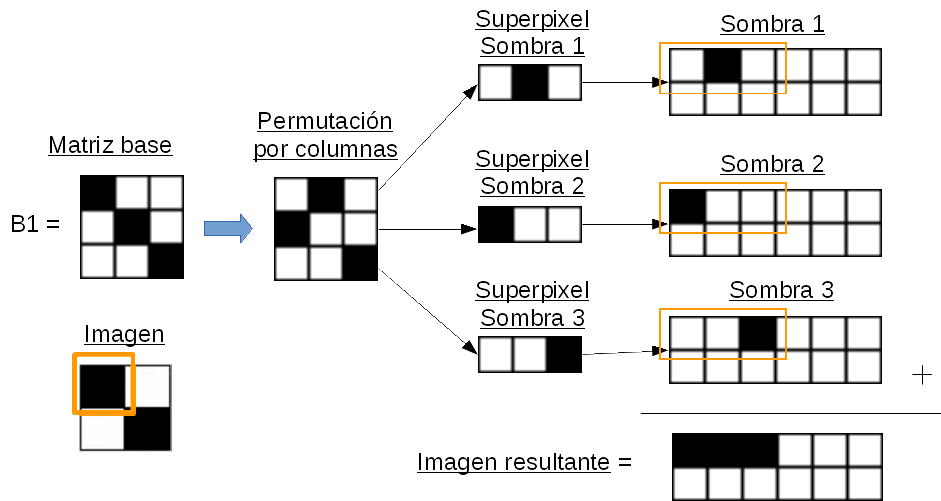
\includegraphics[width=\textwidth]{images/DVCSnegro}
		\caption{Cifrado de un píxel negro}
		\label{fig:cifradoDVCSn}
	\end{subfigure}
	\\[0.5cm]
	\begin{subfigure}[t]{0.9\textwidth}
		\centering
		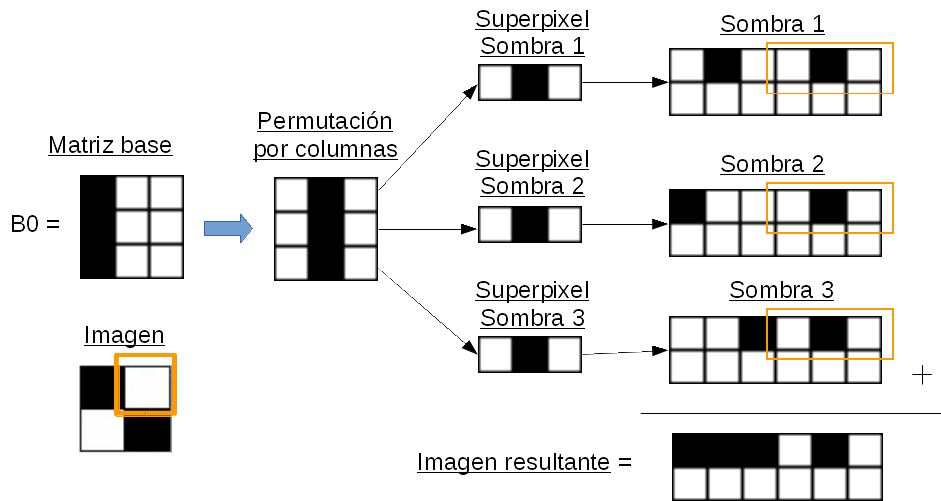
\includegraphics[width=\textwidth]{images/DVCSblanco}
		\caption{Cifrado de un píxel blanco}
		\label{fig:cifradoDVCSb}
	\end{subfigure}
	\caption{Ejemplos de cifrado con DVCS}
	\label{fig:ejemplosDVCS}
\end{figure}

\newpage
\subsection[PVCS]{Probabilistic Visual Cryptographic Scheme}
El algoritmo PVCS es una variante de VCS en la cual el número de píxeles negros
y blancos de un superpíxel no es determinista, sino que viene dado por una
probabilidad (de ahí su nombre). Esto quiere decir que en un superpíxel negro de
la imagen resultado habrá \textbf{probablemente} más píxeles negros y blancos, y
al contrario en el caso de un superpíxel blanco.

Esto tiene sus ventajas e inconvenientes. Por un lado permite que la imagen
resultante tenga la misma resolución que la original, y por otro lado es más
difícil conseguir un contraste adecuado para apreciar con claridad el secreto,
debido a que siempre hay cierta probabilidad de que un píxel blanco termine
siendo negro o de que un píxel negro termine siendo blanco. En la figura
\ref{fig:cifradoPVCSres} se muestra un ejemplo en el que ocurre esto último.

\subsubsection{Pseudocódigo}
\begin{algorithm}[H]
	\KwIn{\\Una imagen I secreta de $W\times H$\\Las matrices base $B_0$ y $B_1$}
	\KwResult{\\N sombras $S_i$ de tamaño $W\times H$}

	\For{all pixel $px$ in I}{
		\eIf{$px$ == blanco}{
			1. Seleccionar una columna $C_j$ aleatoria de $B_0$ (con
			$j\in[0,m-1]$)\;

			2. Añadir el píxel i-ésimo $p_i$ de $C_j$ ($n$ píxeles)
			al superpíxel (1 píxel) de la i-ésima sombra $S_i$\;
		}{
			1. Seleccionar una columna $C_j$ aleatoria de $B_0$ (con
			$j\in[0,m-1]$)\;

			2. Añadir el píxel i-ésimo $p_i$ de $C_j$ ($n$ píxeles)
			al superpíxel (1 píxel) de la i-ésima sombra $S_i$\;
		}
	}
	\Return{$[S_1,S_2,\cdots,S_N]$}
	\caption{PVCS}
	\label{alg:PVCS}
\end{algorithm}
\newpage
\subsubsection{Ejemplos}
\begin{figure}[ht]
	\centering
	\begin{subfigure}[t]{0.6\textwidth}
		\centering
		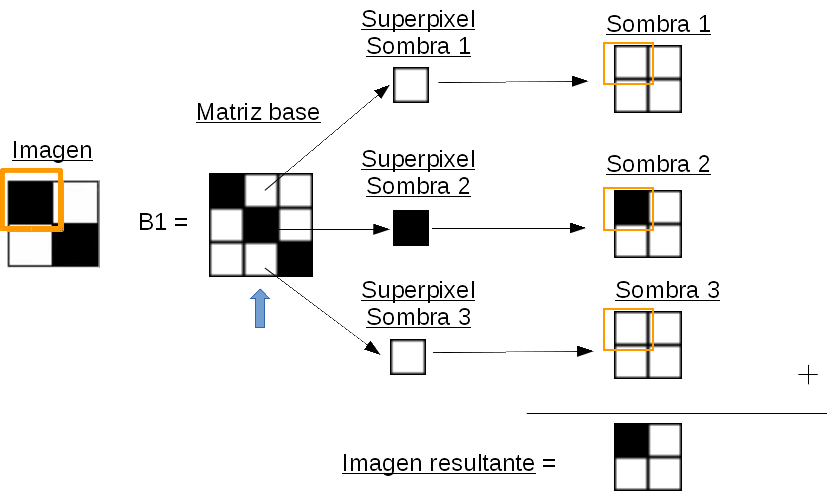
\includegraphics[width=\textwidth]{images/PVCSnegro}
		\caption{Cifrado de un píxel negro. Hay una probabilidad de 3/3
		de escoger un píxel negro.}
		\label{fig:cifradoPVCSn}
	\end{subfigure}
	\hspace{0.5cm}
	\begin{subfigure}[t]{0.3\textwidth}
		\centering
		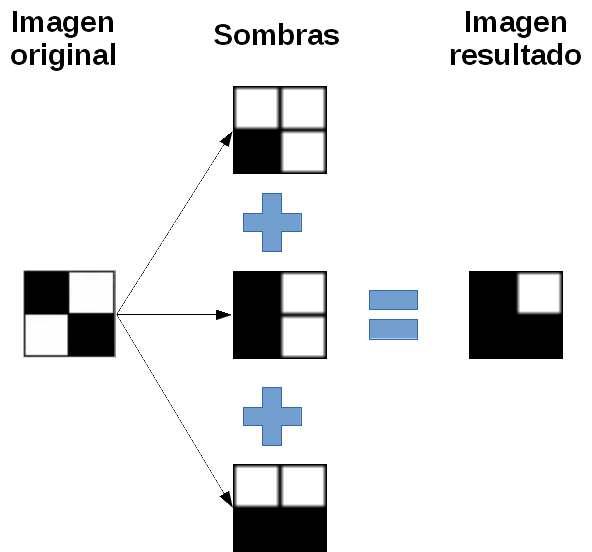
\includegraphics[width=\textwidth]{images/PVCSfallo}
		\caption{Resultado de la superposición de las tres sombras. Se
			observa que un píxel blanco ha terminado siendo negro}
		\label{fig:cifradoPVCSres}
	\end{subfigure}
	\\[0.5cm]
	\begin{subfigure}[t]{0.6\textwidth}
		\centering
		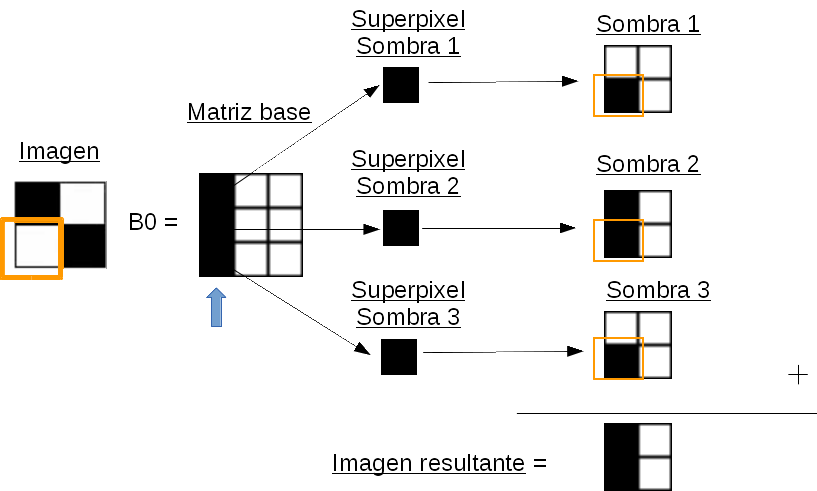
\includegraphics[width=\textwidth]{images/PVCSblanco}
		\caption{Cifrado de un píxel blanco. Hay una probabilidad de 2/3
		de coger un píxel blanco (1/3 de equivocarse).}
		\label{fig:cifradoPVCSb}
	\end{subfigure}
	\caption{Ejemplos de cifrado con PVCS}
	\label{fig:ejemplosPVCS}
\end{figure}
\subsection{Matrices base}
\label{sec:matrices_base}
Como hemos comentado anteriormente, las matrices base son unas matrices binarias
que determinan el comportamiento de los algoritmos VCS. Éstas matrices tienen
que tener dimensión $N\times m$, dónde $N$ es el número de sombras en un esquema
$(K,N)$ y $m$ es el \textsl{factor expansión}, que determinará por cuantos
píxeles se representará un píxel de la imagen original en los superpíxeles de la
imagen resultado, en el caso del algoritmo DVCS.

Además de esto, han de cumplir dos condiciones:
\begin{enumerate}
	\item \textbf{Condición de contraste}[\ref{eq:cond_contraste}] \textsl{El
		número de píxeles negros de un superpíxel negro es mayor que el
		de un superpíxel blanco}. Esto asegura que en la imagen
		resultante se puedan distinguir los superpíxeles negros de los
		blancos.
	\item \textbf{Condición de seguridad}[\ref{eq:cond_seguridad}]: \textsl{El
		número de píxeles negros es el mismo para cualquier superpixel
		resultante de la superposición de $K-1$ sombras o menos}. Esto
		asegura que si se tienen menos de $K$ sombras, no se obtiene
		ninguna información sobre el secreto.
\end{enumerate}

Si definimos la operación $OR(B|r)$ como el vector resultante de realizar la
operación \textsl{or} por columnas, a $r$ filas cualesquiera de la matriz $B$. Y
definimos la operación $H(\cdot)$ como la distancia de hamming (el número de 1s
del vector). Podemos definir las restricciones anteriores mediante las
siguientes ecuaciones:

\begin{align}
	&\begin{cases}
		H(OR(B_0|r)) \ge (m-l) \\
		H(OR(B_0|r)) \le (m-h) 
	\end{cases}
	\text{, si } r = K
	\label{eq:cond_contraste}
	\\\nonumber
	&\text{Con: } 0 \le l < h \le m
\end{align}

\begin{equation}
	H(OR(B_0|r)) = H(OR(B_1|r)) \: \text{, si } r < K
	\label{eq:cond_seguridad}
\end{equation}

Las constantes $l$ y $m$ determinan respectivamente:
\begin{itemize}
	\item $l$: Número máximo de píxeles blancos en un superpíxel negro
	\item $m$: Número mínimo de píxeles blancos en un superpíxel blanco
\end{itemize}
Por lo que variando las mismas podemos ajustar la calidad da la imagen
resultante.

Como veremos en la sección \refcont{sec:impl.matrices_base}, la generación de
estas matrices es un problema muy complejo (vease \cite{generacion_matrices}).
